\documentclass{article}
% formatting
\usepackage{auxiliary/style_files/arxiv}
\usepackage[utf8]{inputenc} % allow utf-8 input
\usepackage[T1]{fontenc}    % use 8-bit T1 fonts
% cross-referencing
\usepackage{hyperref}
% tables
\usepackage{booktabs}
\usepackage{tabularx}
\usepackage{multirow}
\usepackage{caption} 
\usepackage{float} % for forcing placement
\captionsetup[table]{skip=10pt}
% fonts
\usepackage{amsfonts}
\usepackage{microtype}
% color
\usepackage{color}
\definecolor{verbgray}{gray}{0.9}
% figures
\usepackage{graphicx}
% enumeration
\usepackage{enumitem}
% embedd pdf files
\usepackage{pdfpages}

% code
\usepackage{listings} % https://tex.stackexchange.com/a/53951
\lstnewenvironment{code_search}{
    \lstset{
        backgroundcolor=\color{verbgray},
        frame=single,
        basicstyle=\ttfamily,
        %columns=fullflexible,
        xleftmargin=0cm,
    }
}{}
\setcounter{secnumdepth}{5}

\usepackage{footnote}
\makesavenoteenv{tabular}

\title{Life-Cycle Assessment for Sustainable Aviation}


\author{
    \href{https://orcid.org/0000-0003-4859-2650}
    {
\includegraphics[scale=0.06]{auxiliary/figures/orcid.pdf}
    \hspace{1mm}
    Michael Weinold} \\
	Paul Scherrer Institut\\
	Laboratory for Energy Systems Analysis\\
	Group for Technology Assessment\\
	OSHA/D22\\
    5232 Villigen PSI \\
    Switzerland \\
	\texttt{michael.weinold@psi.ch} \\
}

\date{28. July 2022}

\renewcommand{\headeright}{Doctoral Research Plan}
\renewcommand{\undertitle}{Doctoral Research Plan}

%%% Add PDF metadata to help others organize their library
%%% Once the PDF is generated, you can check the metadata with
%%% $ pdfinfo template.pdf
\hypersetup{
pdftitle={Doctoral Research Plan},
pdfauthor={Michael Weinold},
}

\begin{document}

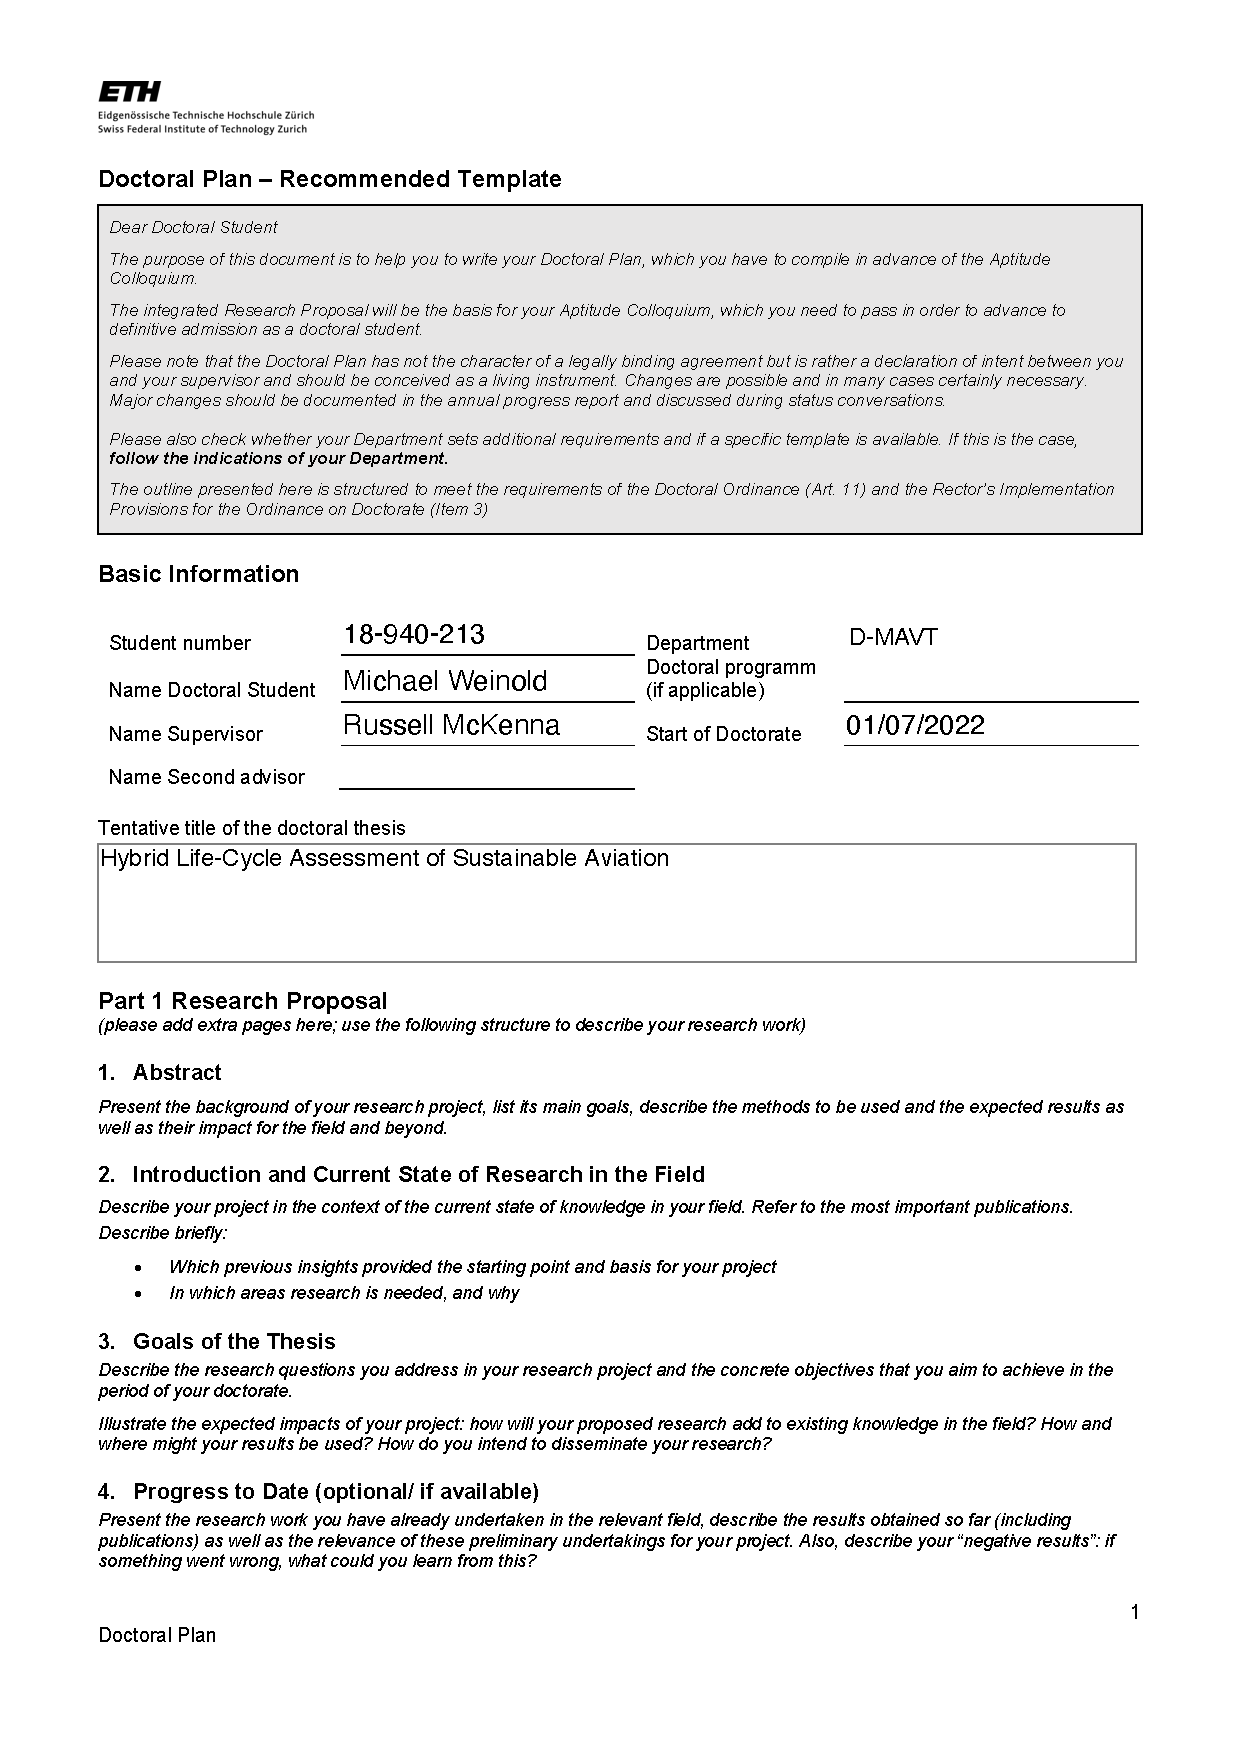
\includepdf[pages=-]{attachments/research_plan_flat.pdf}

\maketitle

\begin{abstract}
	\cite{becattini_role_2021}
\end{abstract}

Attachments:
WISER timeline, WISER sub-project 2 description

\section{Introduction}

Despite the shortcomings of environmental assessments based on pure process-bases life-cycle inventory analysis methods, they are still widely used today. One reason XXX> The methodology required to avoid double counting has not been well formulated. 

    life cycle assessment is \textit{"a tool to assess the potential environmental impacts and resources used throughout a product’s life cycle, i.e. from raw material acquisition, via production and use stages, to waste management"}\cite{noauthor_iso_2006}. Developed in the 1960s \cite{hauschild_life_2018}. 
    
\section{Research Questions}
    
    how are sustainable aviation fuels defined -> CORSIA \cite{prussi_corsia_2021}

    Carbon emissions estimations for individual flights have been available from major flight search providers, including \textit{Google Flights} \cite{holden_google_2021}, \textit{Kayak} \cite{noauthor_kayak_2021} and \textit{SkyScanner} \cite{crosthwaite_how_2021} from 2021. Early studies have shown that the prominent display of carbon emissions can have positive enironmental impact by nudging consumers to choose flights that XXX \cite{amenta_adding_2020}\cite{sanguinetti_nudging_2022}.
    
    However, different methodologies are used to estimate carbon emissions, leading to significant differences in total estimated carbon emissions. For instance, the development team of \textit{Google Flights} changed the calculation methodology to account for direct-air carbon emissions only, disregarding non-carbon emissions \cite{ali_commit_2022}. This has drawn criticism of \textit{"airbrushing emissions"} by environmental non-governmental organizations \cite{hern_google_2022}\cite{rowlatt_google_2022}.
    
    Bombardier published an environmental product declaration (LCA) in 2022: \cite{noauthor_challenger_2022}
    
    
\section{Methods}

    In a first step, a systematic literature review is to be employed to identify all previous attempts at extending life-cycle inventory and avoid double counting. Associated scripts and scientific software will be collected for benchmarking.

    In the next step, a scientific software package is to be developed using best practices from test-driven development \cite{XXX} as well as documentation of scientific software \cite{lee_ten_2018}. The \texttt{pylcaio}\cite{noauthor_pylcaio_2022} script by Agez et al. \cite{agez}\cite{agez} will serve as a starting point. To create the highest level of synergies, matrix operations will be documented using the \texttt{Sphinx}\footnote{\url{https://www.sphinx-doc.org/}} documentation generator and link to relevant literature. The \texttt{Brightway} framework will serve as the computational engine of the package and serve data to XXX. To obtain high computational efficiency on cluster computing environments and alternatively enable practitioners to run calculations on consumer hardware, matrix manipulations will be be optimized. This includes matrix multiplication, row-wise and column-wise manipulations, persistence of matrices to disk and conversion to compressed sparse matrix formats. ...how to move away from heuristics? 
    
    In addition, the \textit{Brightway} package constitutes the computational engine of the WISER digital ecosystem and as such XXXX and, not least of all, to conserve energy.
    
    
    
    Methods:
        software development:
            test driven development
        linear algebra:
            sparse matrices
            sparse matrix compression algorithms
        life-cycle assessment:
            hybridized life-cycle inventory with a sensible method to avoid double counting
            prospective life-cycle assessment
        infrastructure: paralellized on PSI cluster computing hardware
    

\section{Planned Journal Publications}

    test test
    
    For additional context on the timeline of the publications, including mandatory WISER deliverables and proposed work packages, compare the timeline at \url{https://phd.weinold.ch/timeline}.
    
\section{Research in the Context of the WISER Flagship}
    
    A digital ecosystem that simplifies the access to GHG knowledge, project from January 2022 to December 2025.

    
\section{Research in Context of the Department}

    The proposed development of a modular hybridization tool at part of the package \texttt{Brightway} builds on the strong tradition of life-cycle assessment in the Group for Technology Assessment of the Laboratory for Energy Analysis at the Paul Scherrer Institute \footnote{\url{https://www.psi.ch/en/ta/life-cycle-assessment}}. More specifically, life-cycle inventory hybridization is the logical next step connecting work by Aleksandra Kim on global sensitivity analysis of life-cycle assessment \cite{kim_aleksandra-kimgwp_uncertainties_2022}\cite{kim_aleksandra-kimgsa_framework_2021}\cite{paulillo_influential_2021} and work by Romain Sacchi on prospective life-cycle analysis based on integrated assessment models \cite{noauthor_premise_2022}\cite{sacchi_prospective_2022}. The former enables practitioners to understand the drivers of uncertainty, thereby guiding additional life-cycle inventory data collection efforts. The latter 
    However, as illustrated in the introduction, estimates of XXX> Data collection at the process level might be unfeasible due to a lack of data, the 
    Hybridization closes this gap, thereby offering the most accurate assessment to date.
    
    The choice of aviation as the main case study of the proposed tools reflects the importance of the topic laid out in the introduction. It builds on and supplements existing work in the Technology Assessment group by Zipeng Liu and Tom Terlouw \cite{terlouw_large-scale_2022}. It further enables the development of the MAVT lectures \textit{Basics of Air Transport (Aviation I)} and \textit{Management of Air Transport (Aviation II)} \footnote{compare the study plan agreed upon with Prof. McKenna in the appendix} offer an opportunity to XXX.
    
    Due to the multi-method approach combining software development and mathematical optimization with hybrid life-cycle assessment, a number of collaboration opportunities have been identified:
	
	The biggest academic collaboration opportunity identified is the \textit{Cambridge Aviation Impact Accelerator}\footnote{\url{https://www.aiazero.org/}}, founded in 2020 as a collaborative effort of the Whittle Laboratory and Clarence House. With a holistic approach to XXX, including fuels, aircraft and propulsion technologies, airports, non-CO2 emissions, network modelling, broader economic and policy context, and model design, XXX. Research initiatives related to sustainable aviation identified in Switzerland and the European Union usually focus on narrow aspects of efficiency improvements (such as the sub-projects of the EU CleanSky2\footnote{\url{https://www.clean-aviation.eu/clean-sky-2}} program) or on sustainable fuels only (such as the call for research into sustainable fuels\footnote{\url{https://www.bfe.admin.ch/bfe/en/home/research-and-cleantech/funding-program-sweet/calls-for-proposals-overview/sweet-call-2-2022.html}} as part of the SWEET (SWiss Energy research for the Energy Transition) program).
    
    In addition, the Sustainability Commission\footnote{\url{https://mavt.ethz.ch/the-department/organization/bodies-and-committees.html}} of the Department of Mechanical Engineering at ETH Zurich has recently published a draft of their white paper on air transport. The commission suggest the founding of  \textit{"a scientific coalition of the international scientific societies and academic institutions for climate-neutral aviation"} \cite{mazzotti_air_2022}. The details of the proposal and any further action on the part of the the university, the department and research are currently pending further decisions by the commission. However, a supporting role of can be envisioned (LEA TA, ESA?).

\section{Hybrid Life Cycle Assessment}

	What is life-cycle assessment?
	Why is its use in aviation a novelty?
	
	Some recent publications have completely disregarded the impact of life-cycle emissions under the assumption that these would be negligible \cite{brazzola_definitions_2022}.
	
	Why is the use of hybrid life-cycle inventory methods in aviation a novelty?
	
\section{USP}
	
    Existing knowledge within PSI, for instance the recent thesis by Saad \cite{saad_synthetic_2022} and unpublished work by \cite{sacchi_climate-neutral_2022}.

\section{Ideas}

    Connect this to "M2.1: Publication analysing impact of multiple standards and standards implementations in LCA"

    Connect this to "RECCE 2035: Resource to Climate Comparison Evaluator"

	Chris: research and development phase often missed completely in LCA
	Chris: Airbus is using Brightway in future aircraft design
	Chris: knowledge in the group on sustainable fuels (Tom Terlouw?)
	

\section{Questions}

How do the results from Romain's preprint \cite{sacchi_climate-neutral_2022} compare against the new ICAO paper \cite{prussi_corsia_2021}

\newpage
\section{Systematic Literature Review}


    \subsection{Hybrid LCA}
        
        Hybrid life-cycle assessment refers to the combination of two different approaches to building inventory data. 
        
        First ideas in the 80s. The first significant mention of hybrid LCA in review by Lenzen in 2000 \cite{lenzen_errors_2000}.
            
        Why are differences in PLCA so large? One reason: different choice of system boundaries ( compare 2. Method and data 2.1. Hybrid life cycle assessment in \cite{teh_hybrid_2017}
        
        The difference in results between a purely process-based and a hybrid life-cycle assessment is naturally dependent on the parameters listed in section. FIGURE HERE!
        
        The only review of hybrid life-cycle assessment methods identified is provided by Crawford et al. in 2018 \cite{crawford_hybrid_2018}. \cite{}
        
        \begin{table}[H]
            \centering
            \begin{tabularx}{\textwidth}{| X | X | X | X |}
                \hline
                    \textbf{Study} & \textbf{Sector} & \textbf{Methodology} & \textbf{Indicators} \\
                \hline
                    Li et al., 2019 \cite{li_economic_2019} & Resource Extraction & IO + PLCI & CO2, SO2, NOx, soot \\
                \hline
                    Li et al., 2020 \cite{li_life_2020} & Agriculture & EIO + PLCI, MC-based sensitivity analysis & 10 from TRACI v2.1 \\ % . The results show that environmental impact from EIO-based inventory contributes a meaningful fraction of the impact for ozone depletion (67%), respiratory effects (42%), fossil fuel depletion (38%), and smog (28%) (as opposed to process-based inventory)
                \hline
                    Krishnan et al., 2004 \cite{krishnan_using_2004} & Semiconductors & bespoke IO + PLCA & electricity \\
                \hline
                    Wang et al., 2014 \cite{wang_hybrid_2014} & Semiconductors & EIO + LCI (stochiometric approach for chemicals) & human toxicity (cancer), water eutrophication, GWP, etc. \\
                \hline
                    Stokes et al., 2008 \cite{stokes_energy_2009} & Water Supply & EIOLCA tool \footnote{\url{http://www.eiolca.net/}} & CO2, SO2, NOx, soot, etc. \\
                \hline
                    Murray et al., 2008 \cite{murray_hybrid_2008} & Wastewater Treatment & EIOLCA tool \footnote{\url{http://www.eiolca.net/}} & CO2, SO2, NOx, soot, etc. \\
                \hline
                    Teh et al., 2017 \cite{teh_hybrid_2017} & Raw Materials Production & IELab tool \footnote{\url{https://ielab.info/}} & CO2 \\
                \hline
                    Facanha et al., 2006 \cite{horvath_environmental_2006} & Transportation (Land) & EIO + PLCI & CO2, NOx, PM10, CO \\
                \hline
                    Ewing et al., 2011 \cite{ewing_insights_2011} & Transportation (Sea) & EIOLCA tool \footnote{\url{http://www.eiolca.net/}} & CO2eq \\
                \hline
                    Martinez-Corona et al., 2016 \cite{martinez-corona_hybrid_2017} & Electricity (Geotherm.) & THEMIS tool \cite{gibon_methodology_2015} & GWP, etc. \\
                \hline
                    Vasan et al., 2014 \cite{vasan_carbon_2014} & Electronics Manufacturing & EIO + PLCI & CO2eq \\
                \hline
                    Arvesen et al., 2014 \cite{arvesen_life_2014} & Electricity (Wind) & EIO + PLCI & multiple \\
                \hline
                    Yao et al., 2014, \cite{yao_hybrid_2014} & PV Manuf. & EIO + PLCI & multiple \\
                \hline
                    Zhao et al., 2019 \cite{zhao_comparative_2019} & Li-Ion Battery Manuf. & detailed (follow-up) & multiple \\
                \hline
                    Wu et al., 2019 \cite{wu_assessing_2019} & Transportation (Land) & THEMIS tool \cite{gibon_methodology_2015} & CO2eq \\
                \hline
                    Ramaswami et al., 2008 \cite{ramaswami_demand-centered_2008} & Urban Emissions & generic & CO2eq \\
                \hline
                    Chang et al., 2014 \cite{chang_shale--well_2014} & Resource Extraction & generic? & CO2eq, SO2, NOx, CH4 \\
                \hline
            \end{tabularx}
            \caption{Selection of environmental impact studies using a hybrid life-cycle assessment methodology. The search query used to list all relevant studies is listed in section \ref{sub_boolean} in the Appendix. Studies excluded are those older than 5 years with less than 5 citations and those describing sectors deemed too specific (e.g. \textit{"Comparative life cycle assessment of drinking straws in Brazil" \cite{zanghelini_comparative_2020}}. Abbreviations: IO = Input Output Table/Database, PLCI = Process-Based Life-Cycle Inventory Database, MC = Monte-Carlo Technique}
        \end{table}

    \subsection{Life-Cycle Assessment of (Sustainable) Aviation}

\newpage
\section{Progress to Date}

    As per October 2022, the following sub-tasks have been started and/or successfully completed:
    
    \begin{enumerate}
        \item Collection and initial assessment of input/output databases and supply chain information for hybridization. This includes the following databases: \texttt{Exiobase}, \texttt{IEDC}, \texttt{global-fossil-fuel-supply-chain}\footnote{\url{https://github.com/Lkruitwagen/global-fossil-fuel-supply-chain/}}
        \item
            Implementation of \texttt{pylcaio} and \texttt{pymrio} functionality in \texttt{Brightway}.
            \begin{enumerate}
                \item
                    Platform independent testing and debugging setup of \texttt{ecospold2matrix}, \texttt{pymrio}, \texttt{pylcaio} \footnote{\url{https://github.com/michaelweinold/bw_hybrid/blob/master/dev/notebooks}}.
                \item
                    Performance assessment and improvement of existing matrix manipulation and multipilcation algorithms (compare figure \ref{fig:performance}).
                \item
                    Detailed development plan for the refactoring, documentation and implementation of \texttt{pylcaio} functionality in \texttt{Brightway} \footnote{\url{https://github.com/michaelweinold/bw_hybrid/tree/master/.markwhen}}
            \end{enumerate}
        \item
            Migration and upgrade of the existing \texttt{Brightway} API documentation to \texttt{Jupyter Book} \footnote{\url{https://github.com/brightway-lca/brightway-training}} (with \texttt{Thebe} integration) \footnote{\url{https://github.com/brightway-lca/brightway-training/issues/1}} and \texttt{Sphinx} via \url{readthedocs.org}.  \footnote{\url{https://github.com/brightway-lca/brightway-documentation}}. This ensures compliance with the  \textit{Diataxis} documentation framework \footnote{\url{https://diataxis.fr/}}. User-oriented documentation and training materials are now interactive, facilitating. Status: working prototypes completed as part of the \textit{Brightcon 2022} Hackathon \footnote{\url{https://2022.brightcon.link/}}. Further improvements (as part of WISER) pending involvement of external technical writer.
        \item
            Upgrade of \texttt{Brighway} packaging/delivery from \texttt{PyPi} to \texttt{Conda-Forge} to enable platform-specific dependencies \footnote{\url{https://github.com/brightway-lca/brightway2/issues/47}}. This enables user-friendly setup on macOS running on M1 processors with AArch64 ("ARM64") architecture \footnote{\url{https://github.com/brightway-lca/brightway2/issues/46}}. Previously, platform-specific sparse linear algebra solvers required high levels of user intervention during setup with high failure rates \footnote{\url{https://github.com/LCA-ActivityBrowser/activity-browser/issues/705}}. Status: New setup tested, respective GitHub issues closed. Merge of \texttt{conda} recipes into the \texttt{conda-forge} repository completed for first core packages, other packages pending.
    \end{enumerate}

\begin{figure}[h!]
	\centering
	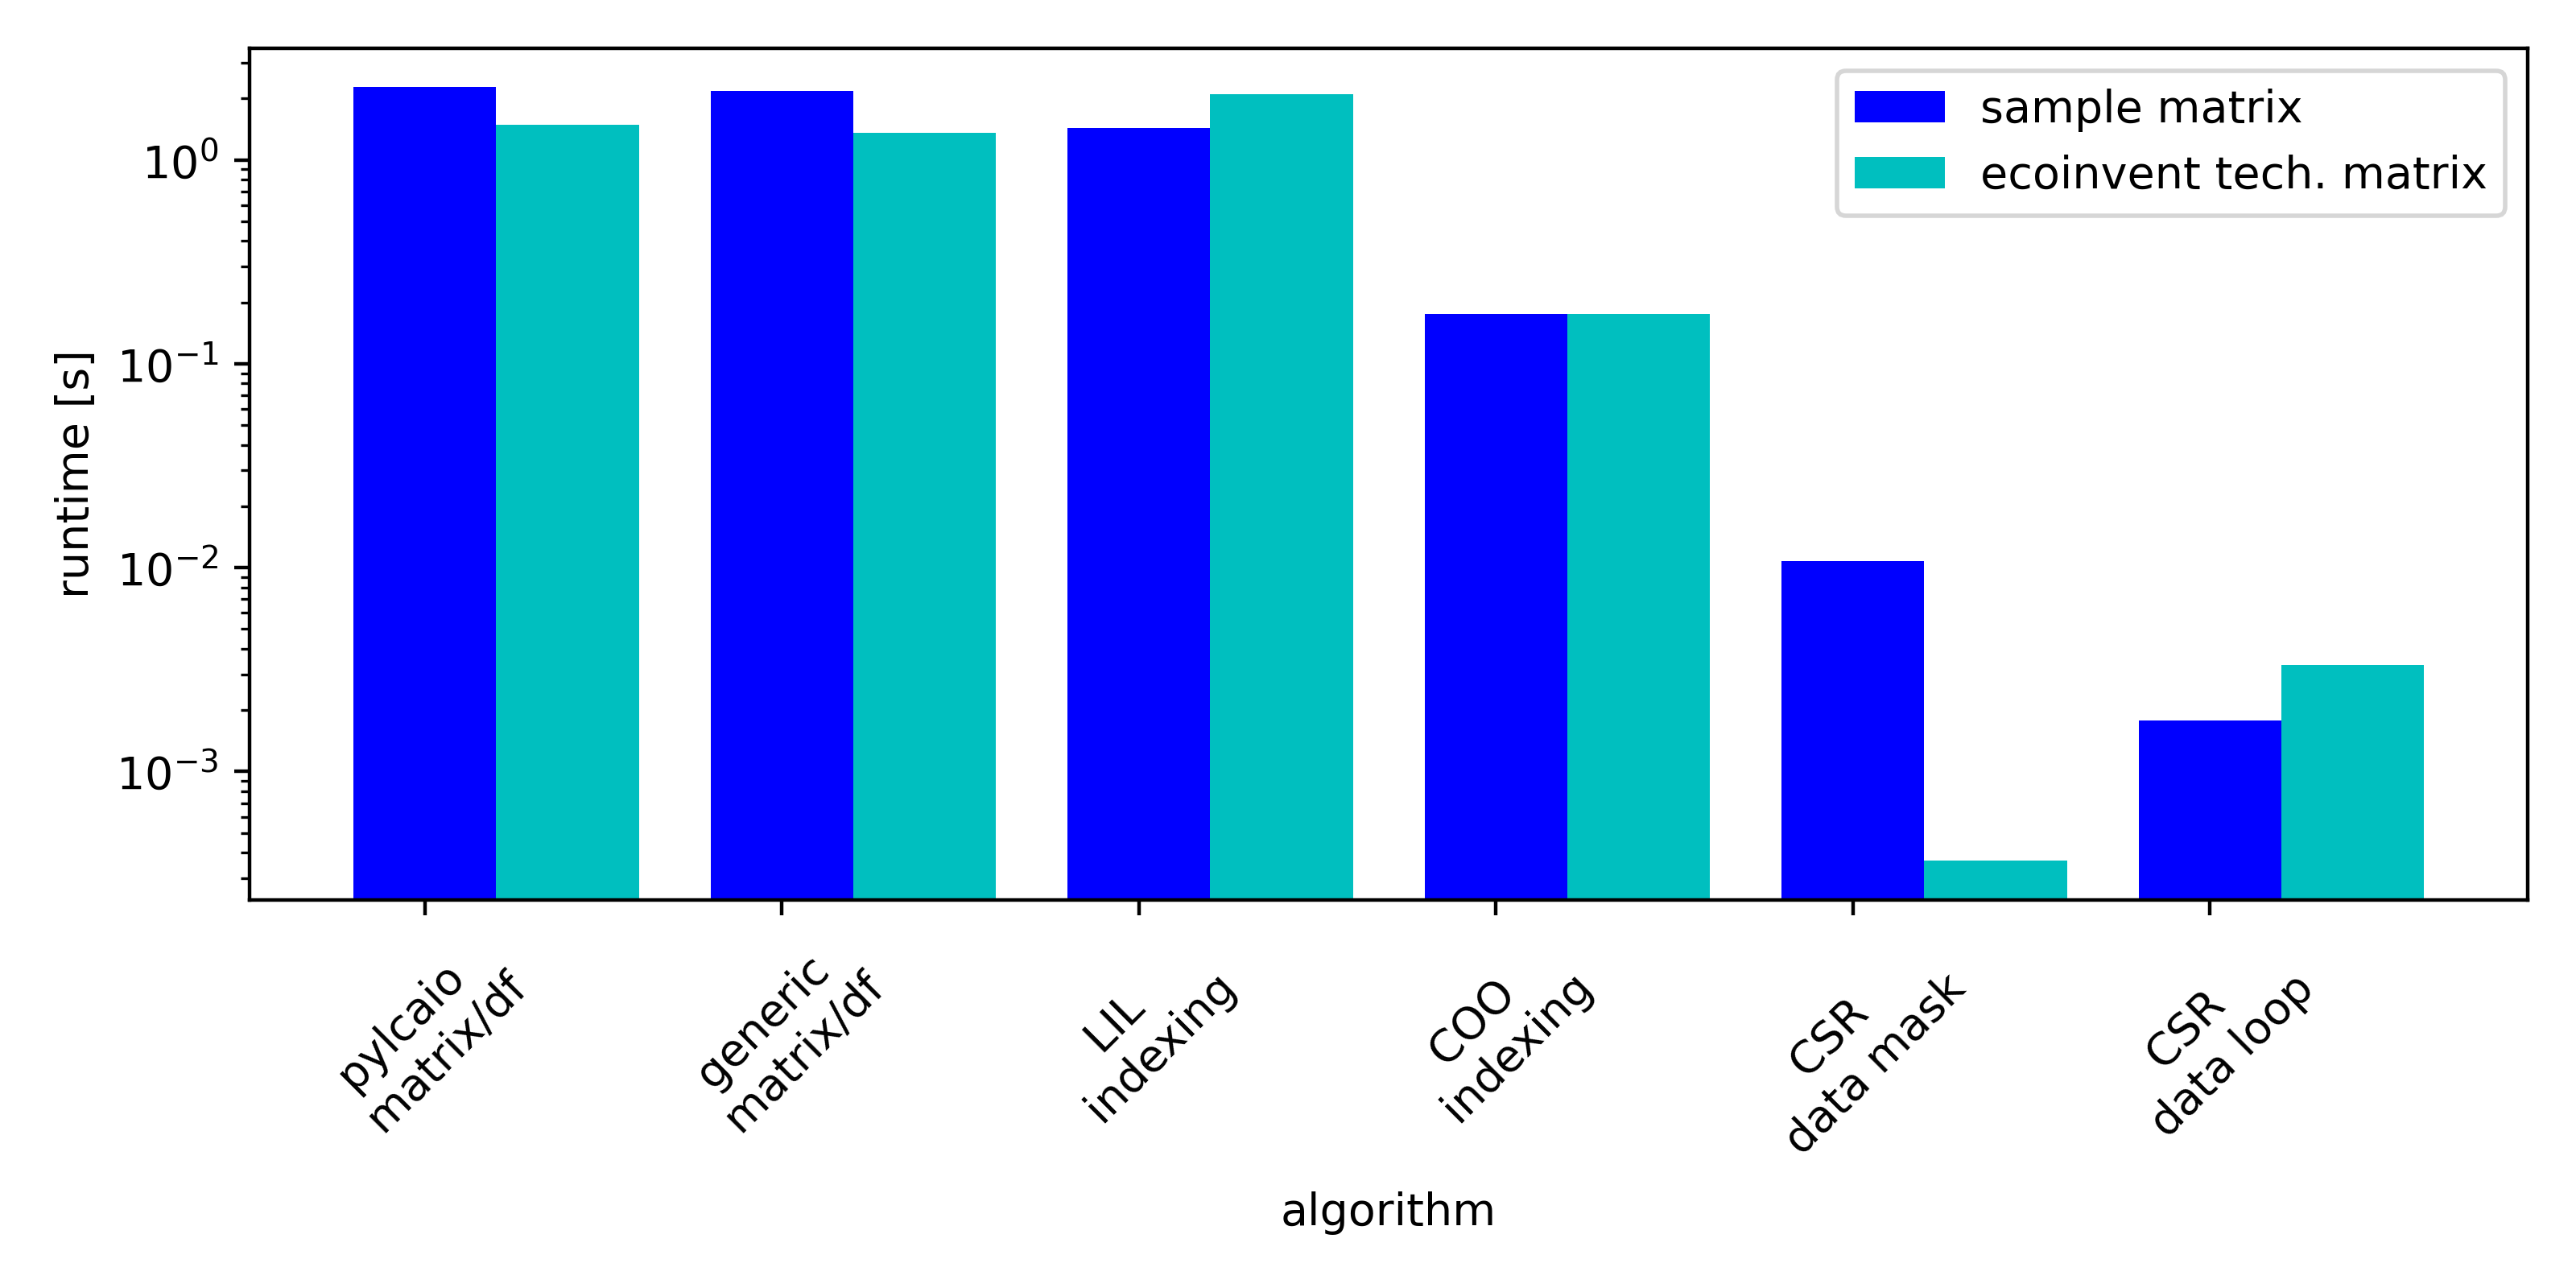
\includegraphics[width=\textwidth]{figures/performance.png}
	\caption{Average runtime of different sparse matrix row-wise manipulation algorithms operating on two different matrices. The most efficient algorithm (\textit{"data mask"}) achieves a runtime improvement of three orders of magnitude over the current implementation in \texttt{pylcaio}. Similar improvements are expected for other parts of the hybridization, based on the current understanding of the code. An overall improvement of at least one, possibly two orders of magnitude Measured using \texttt{\%timeit} (number of loops determined automatically, dependent on convergence of measurement results) under Python 3.10. on an Apple M1 Max platform with 32GB RAM \cite{weinold_github_2022}.}
	\label{fig:performance}
\end{figure}

\newpage
\section{Work Packages}

    Work packages WP1.X are designed to address the aforementioned issues with current solutions for the hybridization of life-cycle inventory. They will also provide the toolkit for investigation of specific technologies in work packages WP3.X. In themselves, they will provide a valuable contribution to the scientific community practicing life-cycle assessment. Building on existing work of the \texttt{Brightway} package, they will be reproducible, XXX, XXX.
    
    Work packages WP2.X are designed to meet the mandatory WISER deliverables of sub-project 2. The improvements in the computational infrastructure are also targeted at streamlining computationally heavy tasks in work packages WP3.X. They will further provide a simplified framework for the technical documentation of scientific code, which will speed up any publications resulting from work packages WP1.X and WP3.X \footnote{Compare, for instance, the \texttt{pvlib} documentation \url{https://pvlib-python.readthedocs.io/en/stable/reference/generated/pvlib.atmosphere.gueymard94_pw.html}}.
    
    Work packages WP3.X build on the toolkit provided by work packages WP1.X and WP2.X. They are designed to answer specific questions related to the field of sustainable aviation. Out of all work packages, they provide the best opportunity for supervision of master's students.

    Note that generic WISER deliverables, such as annual reports and the mid-term review, are not associated with any one work package. For a full list of WISER deliverables, compare "Subproject 2: Computation \& Assessment Toolbox" in the appendix.

    \begin{table}[H]
        \centering
        
        \begin{tabularx}{\linewidth}{
            |>{\hsize=0.25\hsize}X
            |>{\hsize=1.\hsize}X
            |>{\hsize=1.\hsize}X
            |>{\hsize=1.\hsize}X
            |>{\hsize=0.75\hsize}X|
          } % https://tex.stackexchange.com/a/249043
            \hline
                \textbf{\#} & \textbf{Work Package} & \textbf{WISER} & \textbf{Risks} & \textbf{Duration}
            \\
            \hline
        \end{tabularx}
        
        \begin{tabularx}{\linewidth}{
            |>{\hsize=0.25\hsize}X
            |>{\hsize=1.\hsize}X
            |>{\hsize=1.\hsize}X
            |>{\hsize=1.\hsize}X
            |>{\hsize=0.75\hsize}X|
          } % https://tex.stackexchange.com/a/249043
            \hline
                WP1.1
            &
                LCI Hybridization 
            &
                D2.6 (del. month 9) \newline D2.9 (del. month 42)
            &
                affects WP1.2
            &
                11 - 12 months
            \\
            \hline
        \end{tabularx}
        
    \end{table}
    \vspace*{-9pt}
    
    Life-cycle inventory hybridization (augmentation of foreground processes from process-based life-cycle assessment database with additional information from input-output-based database) to increase accuracy of life-cycle assessment. In scope: \textit{Ecoinvent} and \textit{Exiobase}. For other databases, compare W1.3. Associated risks: Heuristics remain the only viable option to avoid double-counting of emissions. A high degree of manual intervention remains a requirement in hybridization, impeding the simple adoption of other databases in WP1.2. No critical risk to downstream work packages.

    \begin{table}[H]
        \centering
        \begin{tabularx}{\linewidth}{
            |>{\hsize=0.25\hsize}X
            |>{\hsize=1.\hsize}X
            |>{\hsize=1.\hsize}X
            |>{\hsize=1.\hsize}X
            |>{\hsize=0.75\hsize}X|
          } % https://tex.stackexchange.com/a/249043
            \hline
                WP1.2
            &
                \texttt{bw\_hybrid} Integration
            &
                D2.6 (del. month 9) \newline D2.9 (del. month 42)
            &
                dependent on WP1.1
            &
                $\sim$ 6 months
            \\
            \hline
        \end{tabularx}
    \end{table}
    \vspace*{-9pt}
    
    Systematic setup and completion of integration and unit tests for code originating from WP1.1. Also includes relevant refactoring required for integration with \textit{Brightway3} and standards proposed in the \textit{Brightway Strategic Development Plan}.  In scope: 80-100\% test coverage, performance assessments of matrix operations and documentation. Associated risks: None, the tests are a requirement for reproducible results. Most tests can be simple \texttt{assert} statements on before-and-after sample matrices.

    \begin{table}[H]
        \centering
        \begin{tabularx}{\linewidth}{
            |>{\hsize=0.25\hsize}X
            |>{\hsize=1.\hsize}X
            |>{\hsize=1.\hsize}X
            |>{\hsize=1.\hsize}X
            |>{\hsize=0.75\hsize}X|
          } % https://tex.stackexchange.com/a/249043
            \hline
                WP1.3
            &
                LCI Hybridization Database Evaluation
            &
                N/A
            &
                affects no other WP
            &
                $\sim$ 6 months
            \\
            \hline
        \end{tabularx}
    \end{table}
    \vspace*{-9pt}
    
    Continuation of initial assessment of input-output databases for integration with existing hybridization infrastructure developed in W1.1/W1.2. If possible, code from WP1.1 will be amended to offer a greater range of options for hybridization. Higher-resolution supply chain databases will be considered. In scope: \textit{Industrial Ecology Dashboard} and associated databases, various regional input-output databases. Associated risks: If nomenclature and conventions of databases differ too greatly, a simple addition to existing \texttt{bw\_hybrid} functionality will be beyond the scope of the work package. In this case, required steps can be documented to ensure that other interested parties can contribute. Even if no other databases can be added, no other downstream work packages are affected.
    
    \begin{table}[H]
        \centering
        \begin{tabularx}{\linewidth}{
            |>{\hsize=0.25\hsize}X
            |>{\hsize=1.\hsize}X
            |>{\hsize=1.\hsize}X
            |>{\hsize=1.\hsize}X
            |>{\hsize=0.75\hsize}X|
          } % https://tex.stackexchange.com/a/249043
            \hline
                WP2.1
            &
                \texttt{Brightway} Documentation Upgrade
            &
                D2.6
            &
                affects no other WP
            &
                3 months (core)
            \\
            \hline
        \end{tabularx}
    \end{table}
    \vspace*{-9pt}
    
    Upgrade of the existing Brightway documentation in line with the \textit{Brightway Strategic Development Plan}. Release of the documentation for comment to WISER stakeholders and other sub-project leaders. In scope: Upgrade of the documentation to reflect changes as part of WISER sub-project 2, in accordance with \texttt{BEP003}\footnote{\url{https://github.com/brightway-lca/enhancement-proposals/blob/main/proposals/0003.md}}. Associated risks: None identified.
    
    \begin{table}[H]
        \centering
        \begin{tabularx}{\linewidth}{
            |>{\hsize=0.25\hsize}X
            |>{\hsize=1.\hsize}X
            |>{\hsize=1.\hsize}X
            |>{\hsize=1.\hsize}X
            |>{\hsize=0.75\hsize}X|
          } % https://tex.stackexchange.com/a/249043
            \hline
                WP2.2
            &
                GHG Standards in \texttt{Brightway}
            &
                D2.5, M2.7
            &
                affects no other WP
            &
                $\sim$ 6 months
            \\
            \hline
        \end{tabularx}
    \end{table}
    \vspace*{-9pt}
    
    Analysis and comparison of different greenhouse gas assessment standards (carbon footprinting standards) in the Brightway life-cycle assessment software framework. This includes existing implementations and potential differences to novel implementations. Implementation of multiple nomenclature conventions. In scope (as per deliverable): ISO 14067, PAS2050, GHG protocol (scope 1, 2 and 3). Associated risks: None identified.
    
    \begin{table}[H]
        \centering
        \begin{tabularx}{\linewidth}{
            |>{\hsize=0.25\hsize}X
            |>{\hsize=1.\hsize}X
            |>{\hsize=1.\hsize}X
            |>{\hsize=1.\hsize}X
            |>{\hsize=0.75\hsize}X|
          } % https://tex.stackexchange.com/a/249043
            \hline
                WP2.3
            &
                WISER SP1/SP2 API
            &
                D2.7, M2.5
            &
                mandatory deliverable \newline affects all other SPs \newline affects WP2.4
            &
                $\sim$ 6 months
            \\
            \hline
        \end{tabularx}
    \end{table}
    \vspace*{-9pt}
    
    Development of an API interface for \texttt{Brightway} to be used in conjunction with the proposed web-service. Provides an interface to the WISER API developed by sub-project 1. In scope: adaption of existing \texttt{Brightway} infrastructure to allow for full interaction with (currently in development) sub-project 1 API calls. Most likely includes basic LCA calculations, including the choice of dataset, etc. Associated risks: The required changes might be difficult to implement or take an inordinate amount of time. This is also an area of software development in which I have the least experience. Summarily, this work package was identified to carry the highest associated risks, considering also the small benefit rendered to downstream work packages WP3.X, which are more relevant to pulblications vital to the progress of my doctoral studies.
    
    \begin{table}[H]
        \centering
        \begin{tabularx}{\linewidth}{
            |>{\hsize=0.25\hsize}X
            |>{\hsize=1.\hsize}X
            |>{\hsize=1.\hsize}X
            |>{\hsize=1.\hsize}X
            |>{\hsize=0.75\hsize}X|
          } % https://tex.stackexchange.com/a/249043
            \hline
                WP2.4
            &
                \texttt{Brightway} Webservice
            &
                D2.8, M2.6
            &
                mandatory deliverable \newline affects all other SPs 
            &
                $\sim$ 4 months
            \\
            \hline
        \end{tabularx}
    \end{table}
    \vspace*{-9pt}
    
    Enhancement of existing \texttt{Brightway} functionality to provide a web-service to be used as the core "computational engine" of the WISER project. In scope: Streamlining the setup of the packages on a virtual private server and the associated documentation (compare WP2.1). Potentially a \texttt{Docker} container of the required packages. Associated risks: Negligible. Existing infrastructure \footnote{Compare the current Brightway Jupyter-Hub server\url{https://hub.brightway.dev}} and documentation provide an excellent basis. The associated benefit for downstream work packages WP3.X is large, considering the high degree of manual intervention that was still required in the work of Aleksandra Kim \cite{paulillo_influential_2021}.

    \begin{table}[H]
        \centering
        \begin{tabularx}{\linewidth}{
            |>{\hsize=0.25\hsize}X
            |>{\hsize=1.\hsize}X
            |>{\hsize=1.\hsize}X
            |>{\hsize=1.\hsize}X
            |>{\hsize=0.75\hsize}X|
          } % https://tex.stackexchange.com/a/249043
            \hline
                WP3.1
            &
                Sustainable Aviation: \newline Data Collection
            &
                N/A
            &
                affects WP3.2
            &
                $\sim$ 6 months
            \\
            \hline
        \end{tabularx}
    \end{table}
    \vspace*{-9pt}
    
    This includes initial sensitivity/contribution analysis of the underlying data to guide targeted data collection. Early results are to be benchmarked against new industry publications, such as \cite{noauthor_challenger_2022}. In scope: TBD. Associated risks: TBD.
    
    \begin{table}[H]
        \centering
        \begin{tabularx}{\linewidth}{
            |>{\hsize=0.25\hsize}X
            |>{\hsize=1.\hsize}X
            |>{\hsize=1.\hsize}X
            |>{\hsize=1.\hsize}X
            |>{\hsize=0.75\hsize}X|
          } % https://tex.stackexchange.com/a/249043
            \hline
                WP3.2
            &
                Sustainable Aviation: \newline Hybrid LCA
            &
                N/A
            &
                N/A
            &
                $\sim$ 12 months
            \\
            \hline
        \end{tabularx}
    \end{table}
    
    This includes the (potentially prospective, based on \texttt{premise}) life-cycle assessment based on a hybridized inventory. Scope: TBD. Risks: TBD.
    
\section{Time Schedule}

    The proposed schedule associated with this research plan can be viewed as an interactive \textit{Markwhen}\footnote{\url{https://github.com/kochrt/markwhen}} timeline at \url{https://phd.weinold.ch/timeline}.

\newpage
\section{Appendix}

 % https://docs.google.com/spreadsheets/d/14gmD96CXOYMKjaUK2KIvosC4LcfpzAc-_INdCU4LAro/edit#gid=1019504979

    \subsection{Details of Systematic Literature Review Methodology}
    
        The \textit{SALSA} (\textbf{S}earch, \textbf{A}ppraisa\textbf{L}, \textbf{S}ynthesis, \textbf{A}nalysis) framework rationalization introduced by Grant et al. \cite{grant_typology_2009} was utlized in the context of the systematic literature review. Search was conducted through the \textit{Elsevier Scopus Advanced Search} engine \footnote{\url{https://www.scopus.com/search/form.uri?display=advanced}}. Out of the small body of search engines supporting Boolean queries, it was chosen over \textit{Dimensions} \footnote{\url{https://app.dimensions.ai/discover/publication}} and \textit{The Lens} \footnote{\url{https://www.lens.org/lens/search/scholar/structured}} for its ease of use and larger body of indexed publications. Inclusion and exclusion criteria listed in section \ref{subsub_inclusion_exclusion} were used to contruct Boolean search queries listed in section \ref{sub_boolean} to significantly narrow the scope of publications for appraisal. 
        
        \subsubsection{Inclusion/Exclusion Criteria}
        \label{subsub_inclusion_exclusion}
        
            To reduce the number of false positive results, a list of relevant journal subject areas was compiled:
            
\begin{code_search}
F1: PHYS OR ENER OR CENG OR CHEM OR COMP OR EART OR ENVI
F2: F1 OR ECON OR BUSI OR SOCI
F3: PHYS OR ENER OR CENG OR CHEM OR COMP OR EART OR ENVI
\end{code_search}

        
            \begin{table}[H]
                \centering
                \begin{tabularx}{\textwidth}{| X | X |}
                    \hline
                \multicolumn{2}{|l|}{\textbf{(F1.1) Hybrid LCA methods}}  \\
                    \hline
                    \textit{inclusion criteria} & \textit{exclusion criteria} \\
                    \hline
                        hybridization methodology is primary focus \newline
                        process-based life-cycle assessment (PLCA) \newline
                        multi-regional input-output tables (MRIO) \newline
                        environmentally extended IO analysis (EEIOA) \newline
                        specific databases: EXIOBASE, ecoinvent \newline
                        focus on truncation errors and double-counting
                    &
                        journal subject areas
                    \\
                    \hline
                \multicolumn{2}{|l|}{\textbf{(F2.2) Prospective hybrid LCA methods}}  \\
                    \hline
                    \textit{inclusion criteria} & \textit{exclusion criteria} \\
                    \hline
                        all inclusion criteria applied in (2.1) \newline
                        prospective/future hybrid LCA
                    &
                        all exclusion criteria applied in (2.1)
                    \\
                    \hline
                \multicolumn{2}{|l|}{\textbf{(F2.1) LCA specific to (sustainable) aviation}}  \\
                    \hline
                    \textit{inclusion criteria} & \textit{exclusion criteria} \\
                    \hline
                        LCA used as primary method  \newline
                    &
                        LCA target domain too specific \newline (e.g. "aviation catering") \newline
                        fuel input too specific \newline (e.g. "bioethanol production from expired cookies") \newline
                        journal subject areas
                    \\
                    \hline
                \multicolumn{2}{|l|}{\textbf{(F2.2) hybrid LCA specific to (sustainable) aviation}}  \\
                    \hline
                    \textit{inclusion criteria} & \textit{exclusion criteria} \\
                    \hline
                        hybrid LCA used as primary method  \newline
                    &
                        all exclusion criteria applied in (1.1) \newline
                        primary focus on hybrid-electric propulsion \newline
                        (e.g. "Feasibility Study of Hybrid Propulsion")
                    \\
                    \hline
                \multicolumn{2}{|l|}{\textbf{(F3.1) Impact of different GHG standards/implementations in LCA}}  \\
                    \hline
                    \textit{inclusion criteria} & \textit{exclusion criteria} \\
                    \hline
                        comparison of specific assessment frameworks in the context of LCA\newline
                        (i.e. ISO 14040-14044, GHG Protocol, ILCD Handbook, ISO 14067, CDP, GRI, SBTi, PEF/OEF, ESG)
                    &
                        narrow focus on any one framework from the inclusion criteria \newline
                        LCA not in research context
                    \\
                    \hline
                \end{tabularx}
                \caption{Inclusion and exclusion criteria for systematic literature review. Where applicable and possible, these were translated to a Boolean search logic. Compare also section \ref{sub_boolean}. The list of relevant subject areas was compiled by collecting metadata of false positive search results.}
                \label{tab_inclusion_exclusion}
            \end{table}
    
    \subsubsection{Boolean Search Logic}
    \label{sub_boolean}
        
        Note that all upper case strings indicate search operators, all lower case strings indicate search terms. Compare the \textit{Scopus Advanced Search} documentation for a list of operator precedence and syntax definitions \footnote{\url{https://service.elsevier.com/app/answers/detail/a_id/11365/}}. For the inclusion and exclusion considerations that informed the logic, compare table \ref{tab_inclusion_exclusion}.
        
        \paragraph{(F1.1) Hybrid LCA methods}
        \ % required for listings to work with \paragraph{}
        
\begin{code_search}
TITLE-ABS-KEY(
    {hybrid life-cycle}
    OR
    {hybrid life cycle}
    OR
    {hybrid LCA}
)
AND TITLE-ABS-KEY(
    *mrio* or *plca* or eeio or hlca
)
AND TITLE-ABS-KEY(
    {truncation} or {double counting} or {double-counting}
)
AND SUBJAREA(
    PHYS OR ENER OR CENG OR CHEM OR COMP OR EART OR ENVI OR
    ECON OR BUSI OR SOCI
)
\end{code_search}

        \paragraph{(F1.2) Prospective (hybrid) LCA methods}
        \ % required for listings to work with \paragraph{}
        
\begin{code_search}
TITLE-ABS-KEY(
    {hybrid life-cycle}
    OR
    {hybrid life cycle}
    OR
    {hybrid LCA}
)
AND TITLE-ABS-KEY(
    prospect*
)
AND SUBJAREA(
    PHYS OR ENER OR CENG OR CHEM OR COMP OR EART OR ENVI
)
\end{code_search}

        \paragraph{(F2.1) LCA specific to (sustainable) aviation}
        \ % required for listings to work with \paragraph{}
            
\begin{code_search}
TITLE-ABS-KEY(
    {life-cycle assessment}
    OR
    {life cycle assessment}
    OR
    {lca}
)
AND TITLE-ABS-KEY(
    sustainable W/3 aviation
)
AND SUBJAREA(
    PHYS OR ENER OR CENG OR CHEM OR COMP OR EART OR ENVI OR
    ECON OR BUSI OR SOCI
)
\end{code_search}

        \paragraph{(F2.2) Hybrid LCA specific to (sustainable) aviation}
        \ % required for listings to work with \paragraph{}
            
\begin{code_search}
TITLE-ABS-KEY(
    {hybrid life-cycle assessment}
    OR
    {hybrid life cycle assessment}
    OR plca OR *mrio* or eeio
)
AND TITLE-ABS-KEY(
    aviation OR {air transport}
)
AND SUBJAREA(
    PHYS OR ENER OR CENG OR CHEM OR COMP OR EART OR ENVI OR
    ECON OR BUSI OR SOCI
)
\end{code_search}

        \paragraph{(F3.1) Impact of different GHG standards/implementations in LCA}
        \ % required for listings to work with \paragraph{}

\begin{code_search}
TITLE-ABS-KEY(
    {hybrid life-cycle assessment}
    OR
    {hybrid life cycle assessment}
    OR plca OR *mrio* or eeio
)
AND TITLE-ABS-KEY(
    aviation OR {air transport}
)
AND SUBJAREA(
    PHYS OR ENER OR CENG OR CHEM OR COMP OR EART OR ENVI OR
    ECON OR BUSI OR SOCI
)
\end{code_search}

\newpage

\bibliographystyle{IEEEtran}
\bibliography{references}

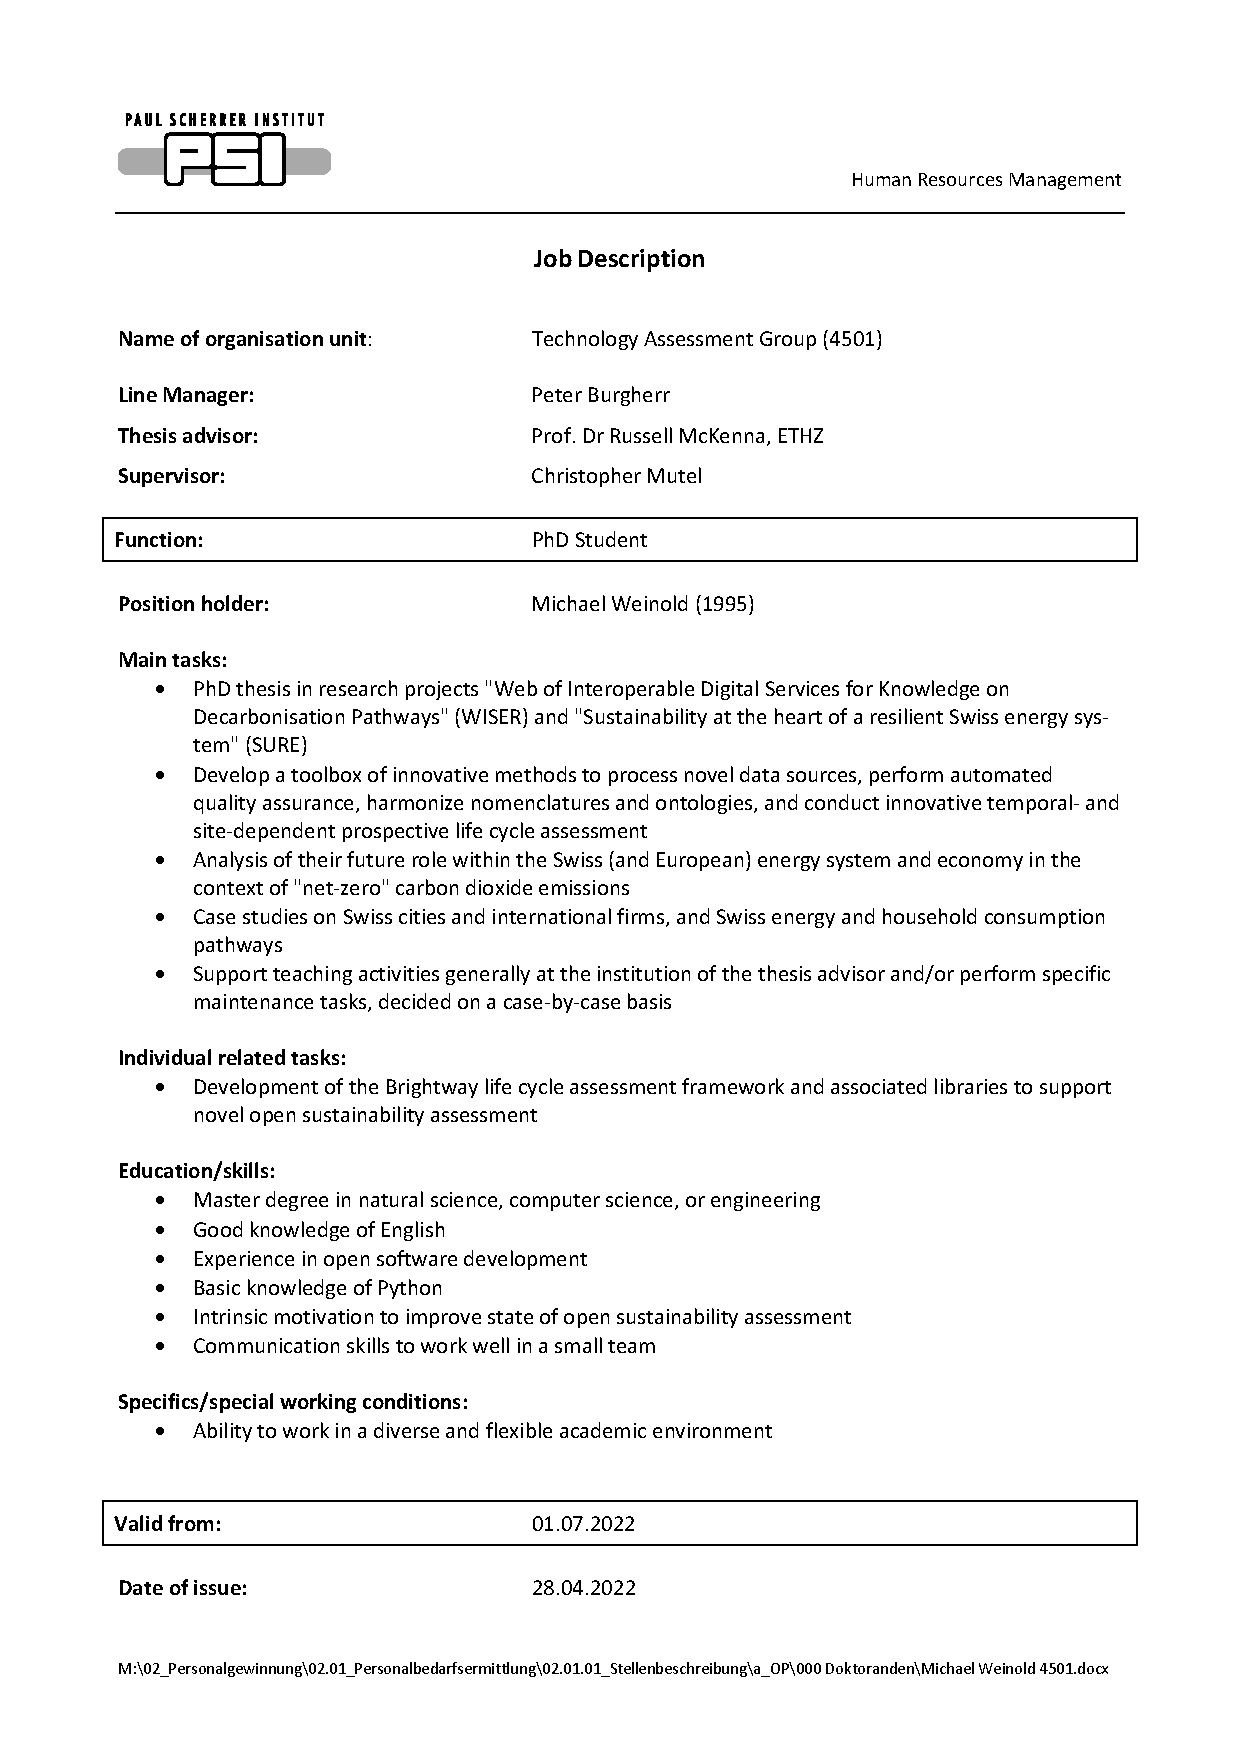
\includepdf[pages=-]{attachments/phd_job_description.pdf}
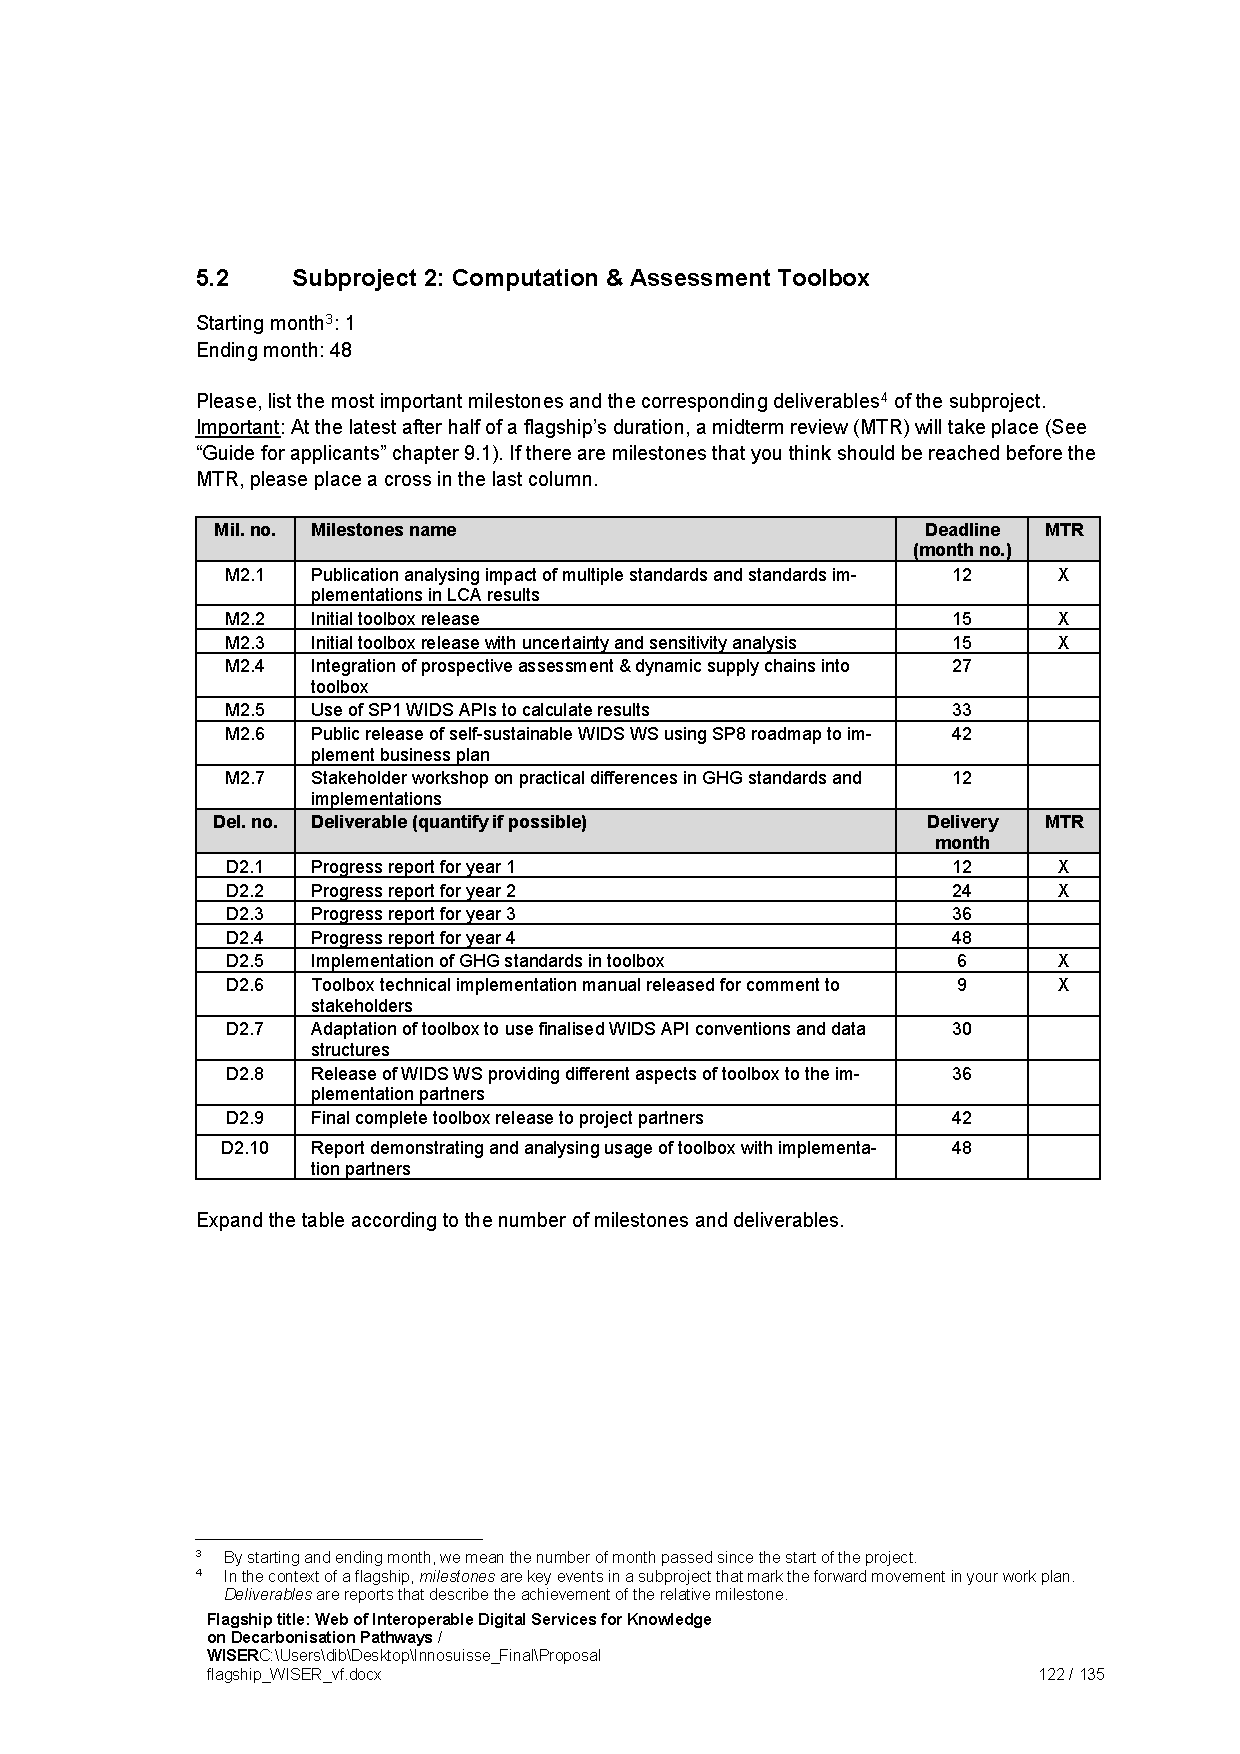
\includepdf[pages=-]{attachments/wiser_sp2_timeline.pdf}
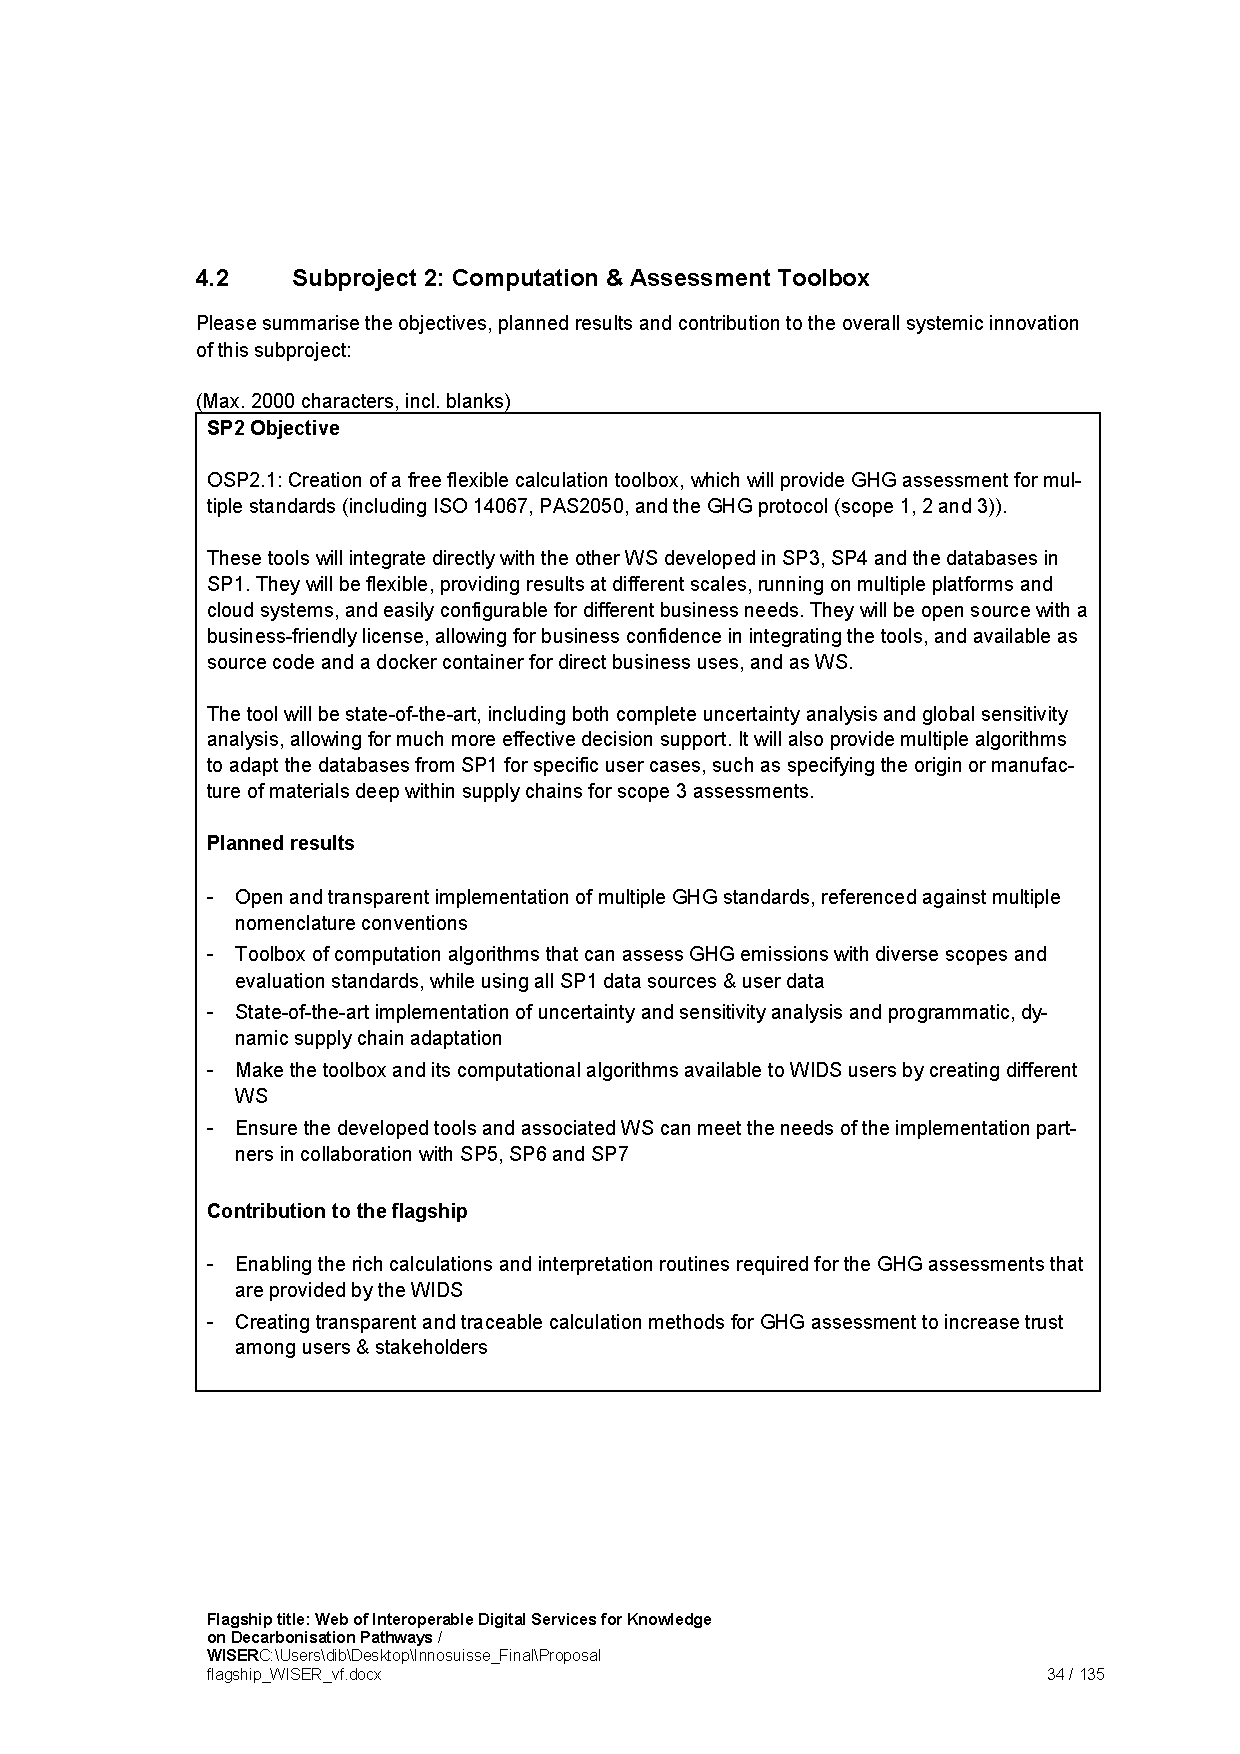
\includepdf[pages=-]{attachments/wiser_sp2_description.pdf}

\end{document}
